\documentclass[12pt]{article}
\usepackage{amsmath}
\usepackage{graphicx}
\usepackage{hyperref}
\usepackage{listings}
\usepackage{color}
\usepackage{pythonhighlight}

\title{Operating System Course Report - First Half of the Semester}
\author{A class}
\date{\today}

\begin{document}

\maketitle
\newpage

\tableofcontents
\newpage

\section{Introduction}
This report summarizes the topics covered during the first half of the Operating System course. It includes theoretical concepts, practical implementations, and assignments. The course focuses on the fundamentals of operating systems, including system architecture, process management, CPU scheduling, and deadlock handling.

\section{Course Overview}
\subsection{Objectives}
The main objectives of this course are:
\begin{itemize}
    \item To understand the basic components and architecture of a computer system.
    \item To learn process management, scheduling, and inter-process communication.
    \item To explore file systems, input/output management, and virtualization.
    \item To study the prevention and handling of deadlocks in operating systems.
\end{itemize}

\subsection{Course Structure}
The course is divided into two halves. This report focuses on the first half, which covers:
\begin{itemize}
    \item Basic Concepts and Components of Computer Systems
    \item System Performance and Metrics
    \item System Architecture of Computer Systems
    \item Process Description and Control
    \item Scheduling Algorithms
    \item Process Creation and Termination
    \item Introduction to Threads
    \item File Systems
    \item Input and Output Management
    \item Deadlock Introduction and Prevention
    \item User Interface Management
    \item Virtualization in Operating Systems
\end{itemize}

\section{Topics Covered}

\subsection{Basic Concepts and Components of Computer Systems}
This section explains the fundamental components that make up a computer system, including the CPU, memory, storage, and input/output devices.

\subsection{System Performance and Metrics}
This section introduces various system performance metrics used to measure the efficiency of a computer system, including throughput, response time, and utilization.

\subsection{System Architecture of Computer Systems}
Describes the architecture of modern computer systems, focusing on the interaction between hardware and the operating system.

\subsection{Process Description and Control}
Processes are a central concept in operating systems. This section covers:
\begin{itemize}
    \item Process states and state transitions
    \item Process control block (PCB)
    \item Context switching
\end{itemize}

\subsection{Scheduling Algorithms}
This section covers:
\begin{itemize}
    \item First-Come, First-Served (FCFS)
    \item Shortest Job Next (SJN)
    \item Round Robin (RR)
\end{itemize}
It explains how these algorithms are used to allocate CPU time to processes.

\subsection{Process Creation and Termination}
Details how processes are created and terminated by the operating system, including:
\begin{itemize}
    \item Process spawning
    \item Process termination conditions
\end{itemize}

\subsection{Introduction to Threads}
This section introduces the concept of threads and their relation to processes, covering:
\begin{itemize}
    \item Single-threaded vs. multi-threaded processes
    \item Benefits of multithreading
\end{itemize}

\begin{figure}[h]
    \centering
    % 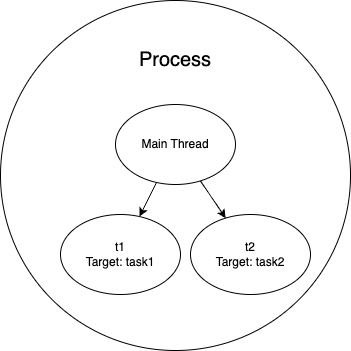
\includegraphics[width=0.5\textwidth]{/a_class/asset/example.png}  % Sesuaikan nama file dan ukurannya
    \caption{Ini adalah gambar contoh dari multithreading.}
    \label{fig:contoh_gambar}
\end{figure}

Seperti yang terlihat pada Gambar \ref{fig:contoh_gambar}, inilah cara menambahkan gambar dengan keterangan.

\subsection{File Systems}
File systems provide a way for the operating system to store, retrieve, and manage data. This section explains:
\begin{itemize}
    \item File system structure
    \item File access methods
    \item Directory management
\end{itemize}

\subsection{Input and Output Management}
Input and output management is key for handling the interaction between the system and external devices. This section includes:
\begin{itemize}
    \item Device drivers
    \item I/O scheduling
\end{itemize}

\subsection{Deadlock Introduction and Prevention}
Explores the concept of deadlocks and methods for preventing them:
\begin{itemize}
    \item Deadlock conditions
    \item Deadlock prevention techniques
\end{itemize}

\subsection{User Interface Management}
This section discusses the role of the operating system in managing the user interface. Topics covered include:
\begin{itemize}
    \item Graphical User Interface (GUI)
    \item Command-Line Interface (CLI)
\end{itemize}


\subsubsection{Fungsi User Interface}
\begin{enumerate}
    \item Meningkatkan Pengalaman Pengguna
    \par \emph{User interface} (UI) yang dirancang dengan baik berfokus pada kemudahan penggunaan dan kenyamanan pengguna dalam berinteraksi dengan sistem. UI yang intuitif, tata letak yang rapi, dan penempatan elemen yang jelas membantu pengguna untuk memahami fungsi aplikasi tanpa perlu belajar berulang kali. Hal ini menciptakan pengalaman yang lebih memuaskan.

    \item Menciptakan Kesan Pertama yang Positif
    \par Kesan pertama merupakan hal yang penting ketika pengguna mulai menggunakan suatu aplikasi atau situs web. UI yang menarik secara visual, responsif, dan terorganisir akan memberikan impresi awal yang positif dan dapat mempengaruhi keputusan pengguna untuk terus menggunakan layanan tersebut.

    \item Meningkatkan Aksebilitas
    \par Desain UI yang baik memperhatikan beragam kebutuhan pengguna, termasuk pengguna dengan keterbatasan fisik atau sensorik. Fitur seperti peningkatan ukuran teks, kontras warna yang sesuai, dan kemampuan untuk menggunakan perangkat bantu memastikan bahwa aplikasi atau sistem dapat diakses oleh lebih banyak orang.

    \item Memfasilitasi Navigasi yang Efisien
    \par UI yang baik membantu pengguna untuk menavigasi aplikasi atau situs web dengan mudah melalui struktur yang konsisten dan logis. Elemen navigasi seperti menu, tombol, dan ikon ditempatkan pada posisi yang strategis, sehingga pengguna tidak perlu membuang banyak waktu mencari fitur atau informasi.

    \item Memudahkan Interaksi Pengguna dengan Produk
    \par UI menjadi perantara antara pengguna dan produk atau layanan. Elemen-elemen visual seperti tombol, ikon, gambar, dan teks menjadi sarana utama yang digunakan pengguna untuk berinteraksi dengan sistem. Desain UI yang baik memastikan interaksi tersebut mudah dan menyenangkan.
\end{enumerate}

\subsubsection{Komponen-komponen User Interface}
Komponen-komponen utama dalam \emph{user interface} (UI) dirancang untuk memfasilitasi interaksi pengguna dengan sistem secara efektif dan intuitif. Berikut adalah komponen-komponen umum dalam UI:

\begin{itemize}

\item \emph{Navigation Bar}

\begin{figure}[h] % Memasukkan gambar
    \centering
    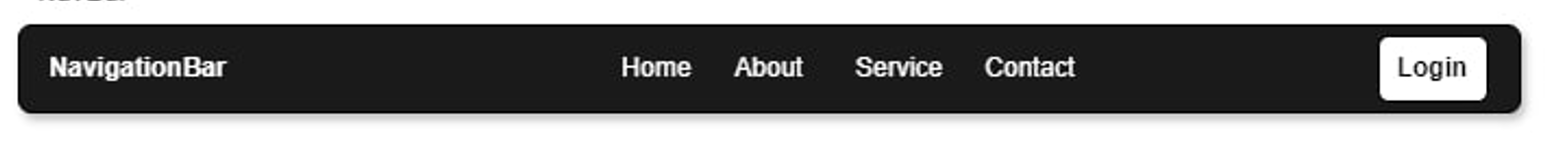
\includegraphics[width=0.5\textwidth]{asset/navbar.png}
\end{figure}

\par Navbar adalah komponen navigasi yang biasanya terletak di bagian atas halaman dan digunakan untuk mengarahkan pengguna ke halaman-halaman penting dalam aplikasi atau situs web. Navbar membantu pengguna menavigasi konten dengan mudah dan cepat.

\par Steve Krug (2005) menjelaskan bahwa navigation bar adalah elemen yang dirancang untuk membantu pengguna berpindah dari satu halaman ke halaman lainnya dengan cara yang paling efisien. Navigation bar yang baik harus mudah ditemukan dan digunakan tanpa perlu berpikir keras.

\item \emph{Buttom}

\begin{figure}[h] % Memasukkan gambar
    \centering
    
\includegraphics[width=0.5\textwidth]{asset/button.png}
\end{figure}

\par Tombol (\emph{Button}) adalah elemen interaktif yang dapat diklik oleh pengguna untuk melakukan suatu tindakan, seperti mengirimkan data, membuka halaman lain, atau menjalankan fungsi tertentu. Tombol memiliki bentuk dan gaya yang mudah dikenali dan diidentifikasi.

\par Ben Shneiderman (2010) menjelaskan bahwa tombol (\emph{button}) adalah elemen dasar dalam antarmuka yang digunakan untuk memicu aksi atau perintah tertentu. Tombol harus dirancang dengan visual yang jelas dan mudah dikenali oleh pengguna, serta memberikan umpan balik yang sesuai setelah diklik.

\item \emph{Form Input} 

\begin{figure}
    \centering
    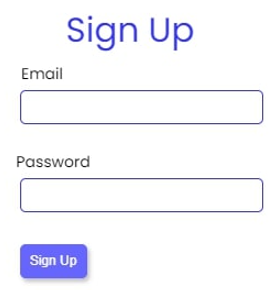
\includegraphics[width=0.5\linewidth]{asset/form.png}
\end{figure}

\par \emph{Form input} adalah elemen di mana pengguna dapat memasukkan informasi ke dalam sistem. \emph{Form input} biasanya digunakan untuk mengumpulkan data dari pengguna, seperti teks, angka, pilihan dari daftar, atau file.

\par Ben Shneiderman (2010) menjelaskan bahwa form input adalah elemen UI yang digunakan untuk memungkinkan pengguna memasukkan data atau informasi ke dalam sistem. Input form harus dirancang agar mudah digunakan, dapat diakses, dan memberikan umpan balik yang jelas kepada pengguna setelah data dimasukkan.

 \item \emph{Card}

 \begin{figure}[h] % Memasukkan gambar
    \centering
    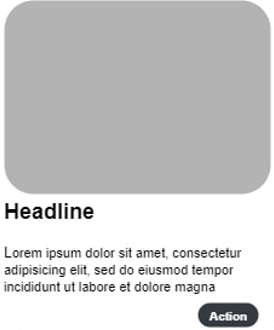
\includegraphics[width=0.5\textwidth]{asset/card.png}
\end{figure}

\par \emph{Card} adalah komponen UI yang biasanya berbentuk kotak persegi atau persegi panjang, yang digunakan untuk menampilkan informasi singkat, media, atau konten dalam bentuk yang rapi dan terstruktur. \emph{Card} memudahkan pengguna untuk melihat beberapa elemen atau konten yang terkait dalam satu wadah.

\par Luke Wroblewski (2011) menjelaskan bahwa \emph{card} adalah elemen UI yang efektif untuk menyajikan informasi dalam potongan kecil dan mudah dicerna, terutama pada perangkat seluler. Dengan menggunakan \emph{card}, konten dapat disajikan secara modular, sehingga pengguna dapat dengan mudah memahami setiap elemen informasi tanpa merasa kewalahan.

\item Modal (\emph{Popup Dialog})

\begin{figure}[h] % Memasukkan gambar
    \centering
    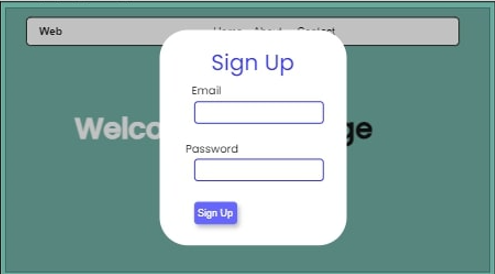
\includegraphics[width=0.5\textwidth]{asset/popUp.png }
\end{figure}

\par Modal adalah kotak dialog yang muncul di atas halaman utama untuk menampilkan informasi penting atau meminta konfirmasi dari pengguna. Modal digunakan untuk interaksi yang tidak mengharuskan pengguna berpindah halaman, sehingga mengurangi gangguan pada alur pengguna.

\par Alan Cooper (2014) menjelaskan bahwa modal adalah jendela dialog yang memblokir interaksi dengan halaman utama hingga pengguna menyelesaikan aksi pada modal tersebut. Modal sering digunakan untuk meminta pengguna mengambil keputusan penting atau memberikan konfirmasi atas tindakan tertentu.

\item \emph{Footer}

\begin{figure}[h] % Memasukkan gambar
    \centering
    
\includegraphics[width=0.5\textwidth]{asset/footer.jpg}
\end{figure}

\par \emph{Footer} adalah area yang terletak di bagian bawah halaman web dan biasanya digunakan untuk menampilkan informasi umum, tautan penting, atau hak cipta. \emph{Footer} berfungsi sebagai penutup halaman dan sering kali menyertakan elemen navigasi tambahan yang tidak terlalu esensial dibandingkan navbar.

\par Steve Krug (2005) menjelaskan bahwa \emph{footer} adalah bagian penting dari halaman web yang memberikan informasi tambahan kepada pengguna, seperti tautan ke halaman kebijakan privasi, syarat dan ketentuan, atau informasi kontak. \emph{Footer} membantu pengguna menemukan informasi penting tanpa harus mencari di seluruh halaman.

\end{itemize}

\begin{thebibliography}{9} 
\bibitem{Shneiderman2016}
Shneiderman, B., Plaisant, C., Cohen, M., Jacobs, S., Elmqvist, N., \& Diakopoulos, N. (2016). \textit{Designing the User Interface: Strategies for Effective Human-Computer Interaction} (6th ed.). Pearson.

\bibitem{Tullis2021}
Tullis, T., \& Albert, B. (2021). \textit{Measuring the user experience: Collecting, analyzing, and presenting usability metrics} (3rd ed.). Morgan Kaufmann.

\bibitem{krug2005}
Krug, S. (2005). \textit{Don't Make Me Think: A Common Sense Approach to Web Usability}. 2nd Edition. New Riders Publishing.

\bibitem{shneiderman2010}
Shneiderman, B. (2010). \textit{Designing the User Interface: Strategies for Effective Human-Computer Interaction}. 5th Edition. Addison-Wesley.

\bibitem{wroblewski2011}
Luke Wroblewski, \emph{Mobile First}. A Book Apart, 2011.

\bibitem{cooper2014}
Alan Cooper, \emph{About Face: The Essentials of Interaction Design}. Wiley, 2014.


\end{thebibliography}

\subsection{Virtualization in Operating Systems}
Virtualization allows multiple operating systems to run concurrently on a single physical machine. This section explores:
\begin{itemize}
    \item Concept of virtualization
    \item Hypervisors and their types
    \item Benefits of virtualization in modern computing
\end{itemize}

\section{Assignments and Practical Work}
\subsection{Assignment 1: Process Scheduling}
Students were tasked with implementing various process scheduling algorithms (e.g., FCFS, SJN, and RR) and comparing their performance under different conditions.
\subsubsection{Group 1}
\begin{python}
    class Process:
    def __init__(self, pid, arrival_time, burst_time):
        self.pid = pid
        self.arrival_time = arrival_time
        self.burst_time = burst_time
        self.completion_time = 0
        self.turnaround_time = 0
        self.waiting_time = 0
\end{python}

\begin{table}[htbp] % Optional: For floating position
    \centering
    \begin{tabular}{|c|c|c|} % Defines number of columns and alignment (c = center, l = left, r = right). '|' creates vertical lines.
    \hline
    Header 1 & Header 2 & Header 3 \\ % Column headers
    \hline
    Row 1, Column 1 & Row 1, Column 2 & Row 1, Column 3 \\ % First row of data
    \hline
    Row 2, Column 1 & Row 2, Column 2 & Row 2, Column 3 \\ % Second row of data
    \hline
    \end{tabular}
    \caption{Your table caption} % Optional: For adding a caption
    \label{tab:your_label} % Optional: For cross-referencing the table
\end{table}
\subsection{Assignment 2: Deadlock Handling}
In this assignment, students were asked to simulate different deadlock scenarios and explore various prevention methods.

\subsection{Assignment 3: Multithreading and Amdahl's Law}
This assignment involved designing a multithreading scenario to solve a computationally intensive problem. Students then applied **Amdahl's Law** to calculate the theoretical speedup of the program as the number of threads increased.

\subsection{Assignment 4: Simple Command-Line Interface (CLI) for User Interface Management}
Students were tasked with creating a simple **CLI** for user interface management. The CLI should support basic commands such as file manipulation (creating, listing, and deleting files), process management, and system status reporting.

\subsection{Assignment 5: File System Access}
In this assignment, students implemented file system access routines, including:
\begin{itemize}
    \item File creation and deletion
    \item Reading from and writing to files
    \item Navigating directories and managing file permissions
\end{itemize}

\section{Conclusion}
The first half of the course introduced core operating system concepts, including process management, scheduling, multithreading, and file system access. These topics provided a foundation for more advanced topics to be covered in the second half of the course.

\end{document}